\chapter{Реализация и экспериментальное исследование}
\section{Реализация алгоритма}
Алгоритм был реализован на языке программирования Java с использованием фреймворка Fork/Join, который хорошо подходит для параллельного исполнения рекурсивных задач.

\subsection{Используемые алгоритмы и структуры данных}
Входной двумерный массив точек остается неизменным, все операции перестановок и модификаций осуществляются на массивах индексов, чтобы избежать лишних копирований памяти.

Для нахождения медианного значения заданного критерия по всем входным точкам используется алгоритм <<Median of medians>> с линейным временем работы.

Большинство процедур в алгоритме изменяют порядок элементов во входном массиве индексов, в связи с чем в параллельной версии возникает задача изолирования памяти.

При каждом вызове \textsc{NDHelperB} копируется нужный отрезок входного массива индексов.
Для восстановления лексикографического порядка во входном массиве используется операция \textsc{merge}.
Операции \textsc{split}, \textsc{merge} и поиск медианы требуют $O(N)$ дополнительной памяти, поэтому они выполняются на буферах, локальных для каждого потока.

Для поддержания упорядоченных множеств <<ступеней>> Парето-фронтов в \textsc{SweepA} и \textsc{SweepB}, описанных в алгоритме Фортена, были реализованы специализированные красно-черное дерево и дерево Фенвика.

Начальная лексикографическая сортировка точек осуществляется с помощью сортировки слиянием.
По мере выполнения лексикографической сортировки заполняется вспомогательный массив $eqComp$ со следующим свойством: если точка $S_i$ совпадает в каждой координате с точкой $S_j$, то $eqComp[i] = eqComp[j]$, если $S_i$ лексикографически меньше $S_j$, то $eqComp[i] < eqComp[j]$.
Эта структура позволяет в дальнейшем сравнивать точки за $O(1)$.

\subsubsection{\textsc{NDHelperA}}
Для реализации описанной во второй главе модификации процедуры \textsc{NDHelperA} необходимо ввести дополнительную структуру, представляющую контекст для отложенного исполнения \textsc{NDHelperB}.

\begin{lstlisting}[float=!h,caption={Вспомогательная структура <<контекст>> для \textsc{NDHelperA}}]
class Context {
    int k;
    int[] compareWith;
    List<Future> futures;
    ...
}
\end{lstlisting}

Добавим в \textsc{NDHelperA} дополнительный аргумент --- список контекстов для отложенного исполнения \textsc{NDHelperB}.

В каждом таком контексте будет храниться:
\begin{itemize}
    \item размерность $k$, по которой будет производиться сравнение;
    \item список индексов $compareWith$ --- точки, с которыми необходимо сравниться;
    \item список $futures$, в который необходимо положить результат отложенного вычисления \textsc{NDHelperB};
\end{itemize}

Если входящий список контекстов не пуст, то до завершения работы \textsc{NDHelperA} необходимо асинхронно запустить выполнение \textsc{NDHelperB} на каждой из частей $L$, $M$ и $H$ в паре с точками из каждого контекста, или на входном отрезке целиком, если деление на части не выполняется.

Результат отложенного исполнения необходимо положить в список $futures$, чтобы у нас была возможность дождаться завершения работы в необходимой нам точке.

В \textsc{NDHelperA(L)} помимо контекстов, переданных сверху, добавляется два новых контекста: первый с отрезком $M$ и списком $waitM$, второй --- с отрезком $H$ и списком $waitH$.
В \textsc{NDHelperA(M)} добавляется контекст с $H$ и списком $waitH$.
Перед запуском \textsc{NDHelperA(M)} мы должны дождаться выполнения задач в $waitM$, а перед запуском \textsc{NDHelperA(H)} --- задач в $waitH$.
Таким образом, все требуемые сравнения точек будут завершены к нужному моменту.

\subsection{Переключение на последовательную версию}
Каждый параллельный вызов \textsc{NDHelperB} при использовании $Fork/Join$ влечет за собой накладные расходы, потому что нам нужно создать новый объект для каждой подзадачи, а также скопировать необходимые отрезки индексов.
Поэтому при достаточно маленьких размерах входных массивов имеет смысл запускать однопоточную версию процедуры.

Был проведен ряд экспериментов при $N=\{10^4, 5\cdot10^4, 10^5\}$, $M=\{3,4,\ldots,15\}$.
В качестве порога в \textsc{NDHelperB} рассматривались степени двойки от $4$ до $1024$.

Лучшие результаты были достигнуты при пороге равном $32$.
Таким образом, если $|L| < 32$ или $|H| < 32$, то запускается однопоточная версия \textsc{NDHelperB(L, H, k)}.

\section{Экспериментальное исследование алгоритма}
Далее будут представлены результаты экспериментального исследования эффективности предложенного алгоритма.

Эксперименты проводились на компьютере с шестнадцатиядерным процессором \textit{AMD Opteron(tm) Processor 6380} с частотой 2.5 ГГц и 4 Гб оперативной памяти.

В качестве тестовых данных использовались искусственно сгенерированные массивы случайных значений. 

Каждая версия алгоритма тестировалась на одной конфигурации входных данных и фиксированном числе потоков исполнения по 25 раз, далее сравнивались минимальное, максимальное и медианное время работы.

\subsection{Сравнение с однопоточной версией алгоритма}
По результатам экспериментов видно, что при больших $N$ достигается неплохой уровень параллелизма.
При $M\leq3$ польза от параллельного исполнения отсутствует, т.к. корневые \textsc{NDHelperB} вызываются с $k=2$, т.е. запускается однопоточная процедура \textsc{SweepB}.

С увеличением $M$ растет количество параллельных подзадач \textsc{NDHelperB}, соответственно прирост в производительности становится более заметным.
Начиная с некоторого значения $M$, глубина дерева исполнения \textsc{NDHelperB} определяется значением $N$ и перестает зависеть от $M$, происходит насыщение всех потоков.

\begin{figure}[h!]
\centering
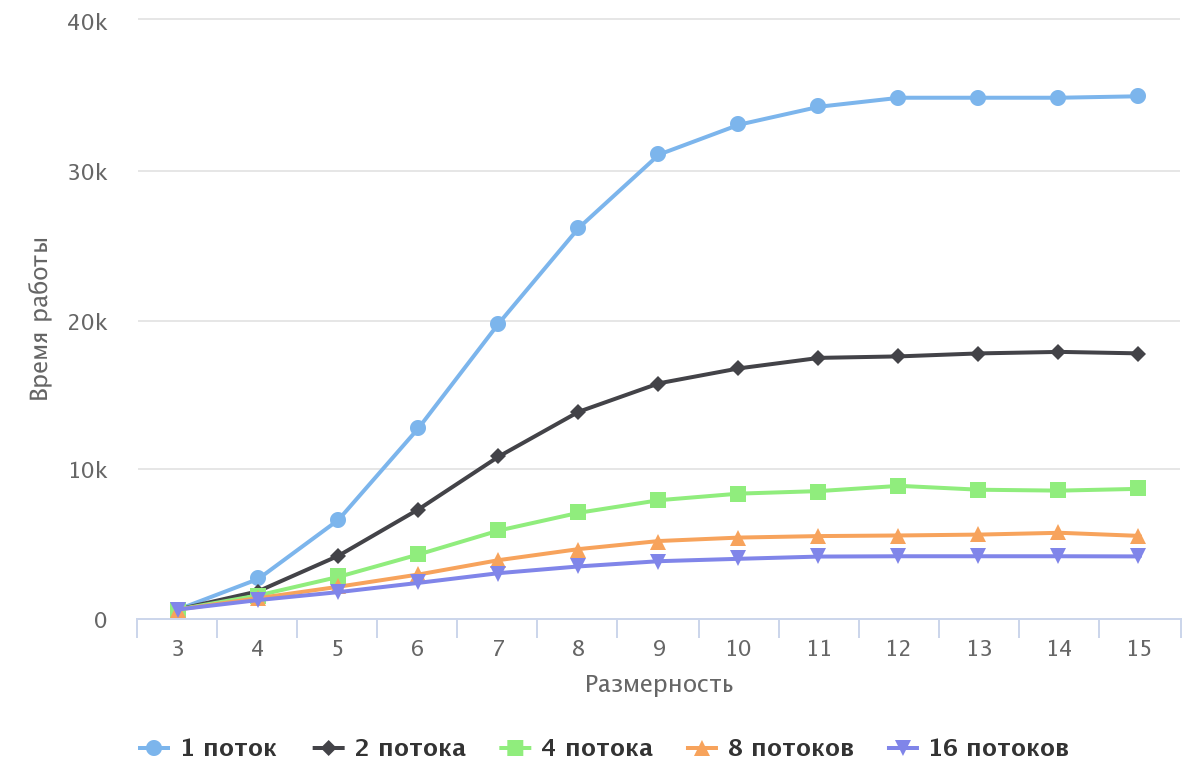
\includegraphics[width=\textwidth]{images/100k.png}
\caption{Медианное время работы\\параллельного алгоритма при $N=10^5$}
\end{figure}

Нам удалось добиться максимального ускорения в $8.47$ раз при $10^5$ точках и 16 потоках.

\begin{table}[h!]
\caption{Время работы алгоритма при $N=10^5$}\label{tab1}
\centering
\begin{tabu}{|*{8}{c|}}
\hline
 & \multicolumn{3}{c|}{Original} & \multicolumn{4}{c|}{Parallel 16 threads}\\
\cline{2-8}
    M & min & max & med & min & max & med & $t_1/t_2$ \\
\hline
    3 & 5.66e+02 & 5.70e+02 & 5.68e+02 & 5.67e+02 & 5.73e+02 & 5.70e+02 & \textbf{1.00}\\ 
    4 & 2.50e+03 & 2.82e+03 & 2.61e+03 & 1.13e+03 & 1.27e+03 & 1.20e+03 & \textbf{2.16}\\
    5 & 6.46e+03 & 6.80e+03 & 6.56e+03 & 1.67e+03 & 1.89e+03 & 1.73e+03 & \textbf{3.79}\\
    6 & 1.26e+04 & 1.28e+04 & 1.27e+04 & 2.28e+03 & 2.45e+03 & 2.35e+03 & \textbf{5.40}\\
    7 & 1.96e+04 & 1.99e+04 & 1.97e+04 & 2.93e+03 & 3.06e+03 & 3.00e+03 & \textbf{6.57}\\
    8 & 2.59e+04 & 2.62e+04 & 2.61e+04 & 3.30e+03 & 3.57e+03 & 3.45e+03 & \textbf{7.57}\\
    9 & 3.08e+04 & 3.12e+04 & 3.10e+04 & 3.69e+03 & 3.91e+03 & 3.80e+03 & \textbf{8.16}\\
    10& 3.28e+04 & 3.32e+04 & 3.30e+04 & 3.85e+03 & 4.03e+03 & 3.96e+03 & \textbf{8.33}\\
    11& 3.41e+04 & 3.45e+04 & 3.42e+04 & 3.99e+03 & 4.24e+03 & 4.11e+03 & \textbf{8.32}\\
    12& 3.46e+04 & 3.51e+04 & 3.48e+04 & 3.98e+03 & 4.25e+03 & 4.13e+03 & \textbf{8.43}\\
    13& 3.46e+04 & 3.51e+04 & 3.48e+04 & 4.00e+03 & 4.36e+03 & 4.13e+03 & \textbf{8.43}\\
    14& 3.46e+04 & 3.50e+04 & 3.48e+04 & 4.01e+03 & 4.43e+03 & 4.13e+03 & \textbf{8.43}\\
    15& 3.47e+04 & 3.52e+04 & 3.49e+04 & 3.95e+03 & 4.25e+03 & 4.12e+03 & \textbf{8.47}\\
\hline
\end{tabu}
\end{table}

\subsection{Сравнение с параллельным алгоритмом Деба}
Для сравнения двух алгоритмов было выбрано относительно небольшое количество точек, т.к. алгоритм Деба из NSGA-II обладает квадратичным временем работы.

По графикам видно, что квадратичный алгоритм лучше масштабируется независимо от $N$. Тем не менее, из-за более плохой асимптотики, он уступает в эффективности предложенному алгоритму при любом количестве потоков от $1$ до $16$. Более того, алгоритм Фортена начинает превосходить шестнадцатипоточный алгоритм Деба уже на четырех потоках.

\begin{table}[h!]
\caption{Сравнение алгоритмов на 16 потоках при $N=10^4$}\label{tab1}
\centering
\begin{tabu}{|*{8}{c|}}
\hline
 & \multicolumn{3}{c|}{Алгоритм Деба} & \multicolumn{4}{c|}{Предложенный алгоритм}\\
\cline{2-8}
    M & min & max & med & min & max & med & $t_1/t_2$ \\
\hline
    3 & 4.80e+02 & 5.03e+02 & 4.91e+02 & 2.69e+01 & 2.72e+01 & 2.70e+01 & \textbf{18.00}\\ 
    4 & 3.29e+02 & 3.83e+02 & 3.53e+02 & 1.16e+02 & 1.41e+02 & 1.34e+02 & \textbf{2.63}\\
    5 & 2.89e+02 & 3.31e+02 & 3.10e+02 & 1.35e+02 & 1.77e+02 & 1.57e+02 & \textbf{1.97}\\
    6 & 2.86e+02 & 3.67e+02 & 3.04e+02 & 1.59e+02 & 2.19e+02 & 1.77e+02 & \textbf{1.72}\\
    7 & 3.07e+02 & 3.89e+02 & 3.23e+02 & 1.65e+02 & 2.19e+02 & 1.86e+02 & \textbf{1.74}\\
    8 & 3.08e+02 & 4.19e+02 & 3.36e+02 & 1.71e+02 & 2.15e+02 & 1.93e+02 & \textbf{1.74}\\
    9 & 3.42e+02 & 3.96e+02 & 3.62e+02 & 1.57e+02 & 2.35e+02 & 1.85e+02 & \textbf{1.96}\\
    10& 3.38e+02 & 4.36e+02 & 3.82e+02 & 1.70e+02 & 2.47e+02 & 1.87e+02 & \textbf{2.04}\\
    11& 3.82e+02 & 5.33e+02 & 4.14e+02 & 1.65e+02 & 2.10e+02 & 1.88e+02 & \textbf{2.20}\\
    12& 3.88e+02 & 4.79e+02 & 4.23e+02 & 1.64e+02 & 2.00e+02 & 1.84e+02 & \textbf{2.30}\\
    13& 4.15e+02 & 4.81e+02 & 4.44e+02 & 1.62e+02 & 2.15e+02 & 1.84e+02 & \textbf{2.41}\\
    14& 4.44e+02 & 5.79e+02 & 4.72e+02 & 1.58e+02 & 2.12e+02 & 1.84e+02 & \textbf{2.57}\\
    15& 4.86e+02 & 5.32e+02 & 5.02e+02 & 1.63e+02 & 2.21e+02 & 1.84e+02 & \textbf{2.73}\\
\hline
\end{tabu}
\end{table}

При большем количестве точек разница в производительности алгоритмов будет прослеживаться более явно из-за разницы в асимптотике и увеличением параллельности нашего алгоритма.

\begin{figure}[h!]
\centering
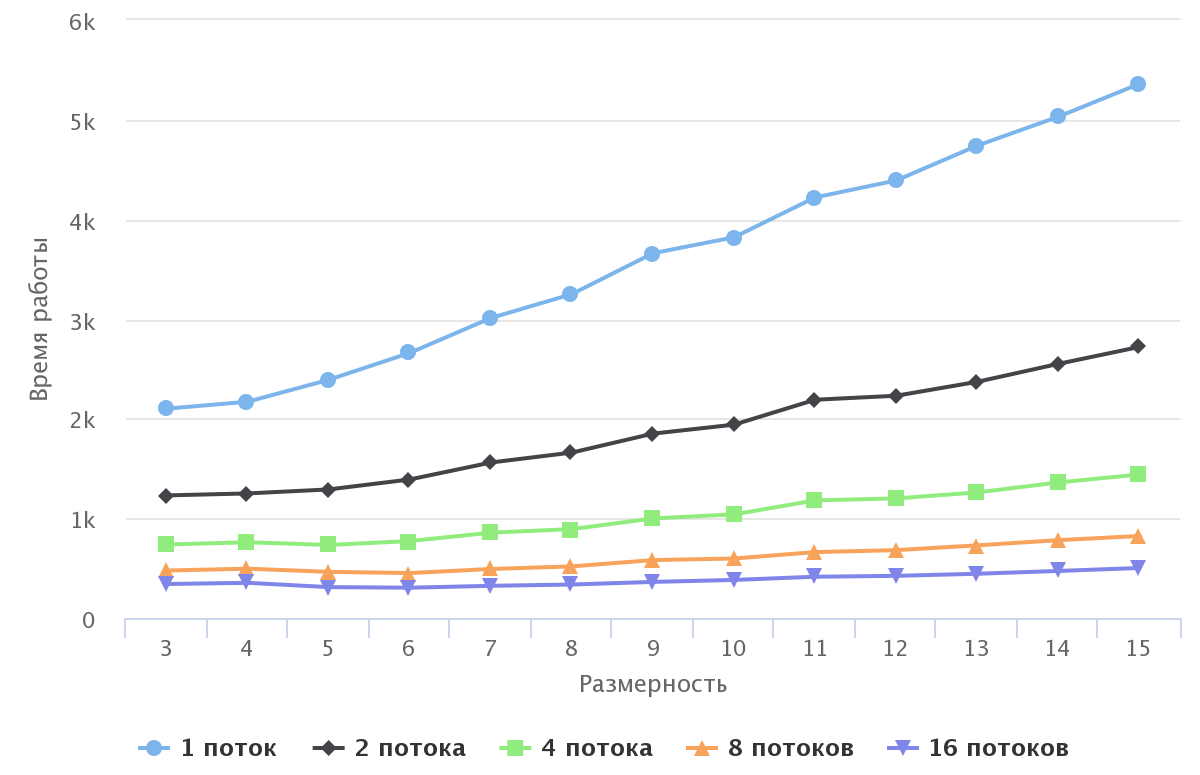
\includegraphics[width=0.95\textwidth]{images/deb10k.png}
\caption{Медианное время работы параллельного алгоритма Деба при $N=10^4$}
\end{figure}

\begin{figure}[h!]
\centering
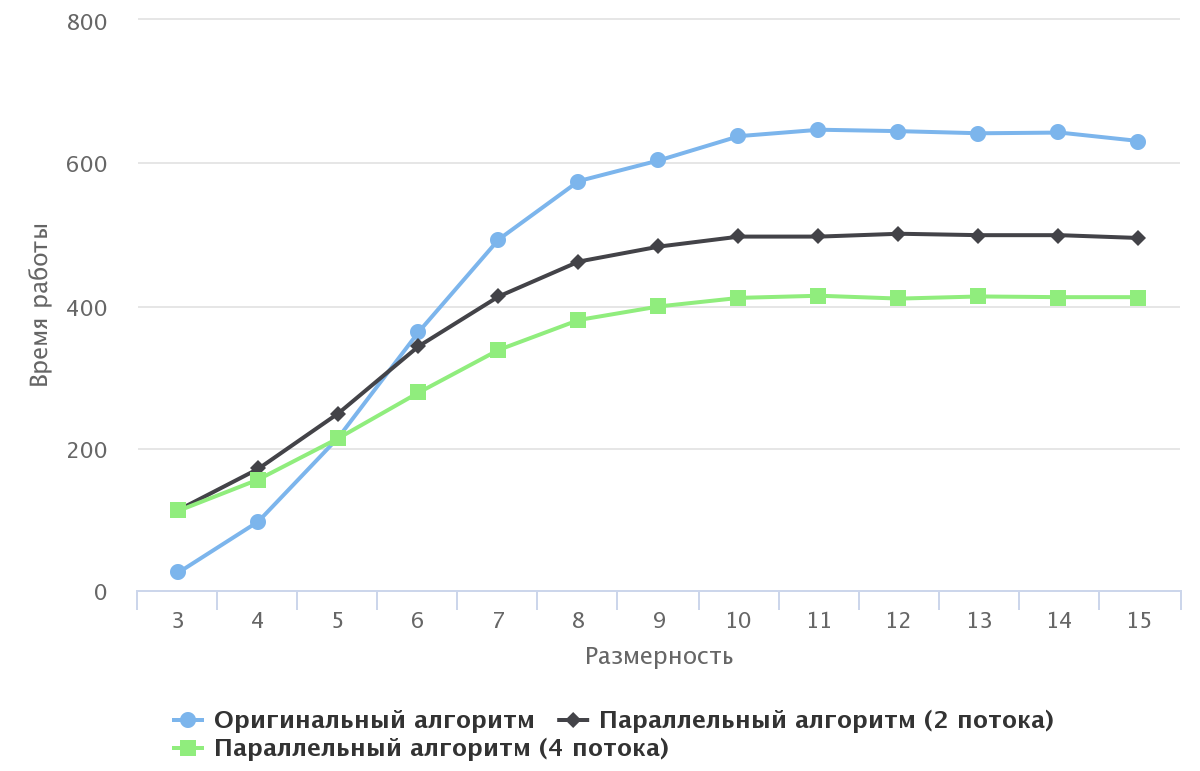
\includegraphics[width=0.95\textwidth]{images/10k.png}
\caption{Медианное время работы параллельного алгоритма Фортена при $N=10^4$}
\end{figure}


\subsection{Оптимизация сортировки}
\subsubsection{Поиск медианы}
Довольно часто вызываемая в данном алгоритме процедура поиска медианы использует в цикле генератор случайных чисел для поиска опорного значения.

Класс $Random$ в языке $Java$ является потоково-безопасным, однако в случае, когда одну и ту же сущность генератора случайных чисел использует сразу несколько потоков исполнения, происходит значительное ухудшение производительности, т.к. потоки делят между собой один ключ внутреннего состояния генератора.

Замена сущности класса $Random$ классом $ThreadLocalRandom$ привела к существенному улучшению экспериментальных результатов алгоритма.

\subsubsection{Уменьшение количества подзадач}
Также большой проблемой на практике является вычислительная стоимость создания новых рекурсивных задач и копирования массивов индексов.

Оптимизация, касающаяся порога переключения \textsc{NDHelperB} на однопоточную версию была описана ранее.

Тем не менее, в процедуре \textsc{NDHelperA} по-прежнему создавались лишние объекты и происходили ненужные копирования памяти при вызове подзадач.
Во избежание подобных накладных расходов часть логики процедуры \textsc{NDHelperB} была продублирована в теле процедуры \textsc{NDHelperA}, а именно, проверка мощностей множеств $L$ и $H$, а также текущей размерности $k$.

Также заметим, что довольно часто среднее подмножество $M$ в \textsc{NDHelperA} и \textsc{NDHelperB}, в которое входят точки с опорным медианным значением, состоит из одного или нескольких элементов. 

В таком случае мы также можем уменьшить количество лишних копирований и создания объектов задач, прикрепив среднее подмножество к меньшему из $L$ и $H$ и продолжить исполнение по схеме алгоритма Фортена.

Вышеописанные оптимизации позволили избавиться от большого количества ненужных дорогостоящих операций.
Таким образом удалось устранить разрыв с оригинальным алгоритмом при малых $M$ и в целом заметно улучшить время работы алгоритма.

\subsubsection{Улучшение SweepA и SweepB}
Изначально для поддержания множеств <<ступеней>> недоминирующих фронтов было реализовано дерево Фенвика.

Встроенный в стандартную библиотеку $TreeMap$ продемонстрировал не самые лучшие результаты из-за накладных расходов при автоупаковке примитивных типов.

В качестве эксперимента было реализовано специализированное красно-черное дерево, заточенное под необходимые нам типы данных.

Применение новой оптимизированной структуры данных также привело к небольшому ускорению работы алгоритма.

\begin{table}[h!]
    \caption{Сравнение структур данных, используемых в \textsc{SweepA} и \textsc{SweepB}. $N=6\cdot10^4$, $4$ потока}
\centering
\begin{tabu}{|*{7}{c|}}
\hline
 & \multicolumn{3}{c|}{Дерево Фенвика} & \multicolumn{3}{c|}{Красно-черное дерево}\\
\cline{2-7}
    M & min & max & med & min & max & med \\
\hline
    3 & 2.33e+02 & 2.39e+02 & 2.34e+02 & 2.27e+02 & 2.31e+02 & 2.28e+02 \\ 
    4 & 5.79e+02 & 6.24e+02 & 5.99e+02 & 5.29e+02 & 5.79e+02 & 5.50e+02 \\
    5 & 1.18e+03 & 1.33e+03 & 1.28e+03 & 1.15e+03 & 1.68e+03 & 1.17e+03 \\
    6 & 2.01e+03 & 2.12e+03 & 2.05e+03 & 1.97e+03 & 2.09e+03 & 2.00e+03 \\
    7 & 2.88e+03 & 3.48e+03 & 2.97e+03 & 2.82e+03 & 3.18e+03 & 2.90e+03 \\
    8 & 3.67e+03 & 3.80e+03 & 3.73e+03 & 3.64e+03 & 3.73e+03 & 3.68e+03 \\
    9 & 4.28e+03 & 4.39e+03 & 4.36e+03 & 4.20e+03 & 4.33e+03 & 4.29e+03 \\
    10& 4.49e+03 & 4.70e+03 & 4.55e+03 & 4.32e+03 & 4.54e+03 & 4.42e+03 \\
\hline
\end{tabu}
\end{table}

\subsection{Анализ модификации NDHelperA}
Несмотря на доказанную теоретическую эффективность, на практике преобразование процедуры \textsc{NDHelperA} имеет довольно узкую область применения.

Это связано с относительно небольшим количеством процессоров, на которых проводилось тестирование.

Как уже было замечено во второй главе, при больших $N$ и начиная с определенной размерности $M$, вызовы \textsc{NDHelperB} производят достаточное количество подзадач, чтобы загрузить работой все свободные процессоры, поэтому предлагаемая модификация \textsc{NDHelperA} не имеет смысла и негативно сказывается на общем времени работы сортировки.

Тем не менее, нам удалось продемонстрировать улучшение времени работы алгоритма при использовании асинхронных вызовов на 32 потоках исполнения при малых $M = \{3,4,5\}$.

Предполагается, что с увеличением количества процессоров мы сможем улучшить степень параллельности алгоритма для малых $M$ и $N$.

\begin{table}[h!]
    \caption{Ускорение при модификации \textsc{NDHelperA}, $N=10^5$}
\centering
\begin{tabu}{|*{7}{c|}}
\hline
 & \multicolumn{3}{c|}{Асинхронная версия} & \multicolumn{3}{c|}{Последовательная версия}\\
\cline{2-7}
    M & min & max & med & min & max & med \\
\hline
    3 & 3.98e+02 & 4.09e+02 & 4.05e+02 & 4.44e+02 & 4.46e+02 & 4.45e+02 \\ 
    4 & 1.26e+03 & 1.38e+03 & 1.33e+03 & 1.35e+03 & 1.47e+03 & 1.42e+03 \\
    5 & 1.61e+03 & 1.86e+03 & 1.75e+03 & 1.87e+03 & 2.04e+03 & 1.95e+03\\
\hline
\end{tabu}
\end{table}

\section{Выводы по главе}
В данной главе были описаны детали реализации, а также проведено экспериментальное исследование предлагаемого алгоритма.

По его результатам можно заключить, что предложенный алгоритм обладает неплохой степенью параллельности и демонстрирует хорошее время работы при различных размерах входных данных.
